\documentclass[10pt]{article}

%\usepackage{hyperref}
\usepackage{alltt}
\usepackage{natbib}
\usepackage{graphicx}
\usepackage{url}
\usepackage{fancyhdr}
\pagestyle{fancy}
%\usepackage{trust}
\usepackage{subfigure}
\usepackage{ifthen}

\usepackage{tikz}
\usetikzlibrary{arrows,shadows}
\usepackage[underline=false]{pgf-umlsd}

\lhead{ArmoredSoftware}
\rhead{Trust in the Cloud}
\lfoot{\copyright The University of Kansas, 2013}
\cfoot{\thepage}


\newboolean{submission}  %%set to true for the submission version
\setboolean{submission}{false}
%\setboolean{submission}{true}
\ifthenelse
{\boolean{submission}}
{ \newcommand{\todo}[1]{ } } % hide todo
{ \newcommand{\todo}[1]{ % show todo
   \marginpar{\raggedright\footnotesize{#1}}
               }}
\newcommand{\squash}{\parskip=0pt\itemsep=0pt}

\parskip=\medskipamount
\parindent=0pt


\bibliographystyle{abbrvnat}

\title{ArmoredSoftware: Trust in the Cloud}
\author{Perry Alexander \and Andy Gill \and Prasad Kuklarni \and Leon
  Searl \\
Information and Telecommunication Technology Center \\
The University of Kansas \\
\url{{palexand,andygill,prasadk,lsearl}@ku.edu}}

\begin{document}

%\maketitle
%\tableofcontents
%\listoffigures
%\listoftables

\begin{abstract}
  \textsc{ArmoredSoftware} is ...
\end{abstract}

\section{Introduction}

The objective of \textsc{ArmoredSoftware} is to \emph{provide a portable
trusted computing capsule for applications executing in the cloud}.
This capsule, referred to as \emph{armor}, provides three major
functions:

\begin{description}
  \parskip=0pt\itemsep=0pt
\item[Appraisal] -- Request and assess measurement information from
  the operational environment and other armored components.
\item[Measurement] -- Gather run-time measurement information from its
  application
\item[Attestation] -- Assemble and deliver evidence to appraisers in a
  manner that assures measurement integrity
\end{description}

\noindent and is based on concepts from \citet{Coker::Principles-of-R}. 

Figure~\ref{fig:architecture} graphically depicts the major
architectural components of a protected application.  The
\emph{application} is the application to be protected by the
infrastructure.  The \emph{measurement} component performs measurement
operations on the running application while the \emph{attestation}
component gathers measurements and delivers them with cryptographic
assurance of integrity and confidentiality.  The \emph{appraisal}
component requests information from the environment and other
components to assess the overall operational environment.
\emph{Access control} governs access to all critical resources in the
protected application to assure secrets are preserved and enforce
information flow restrictions.

\begin{figure}
  \centering
  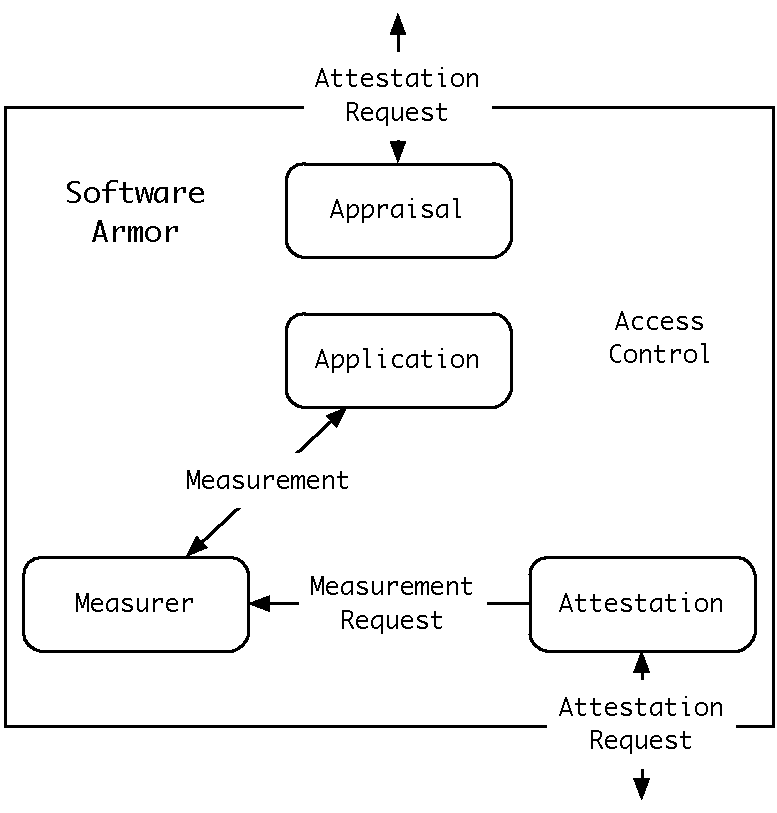
\includegraphics[width=0.5\textwidth]{figures/architecture.pdf}
  \caption{\textsc{ArmoredSoftware} component architecture showing
    major components of the remote attestation process.}
  \label{fig:architecture}
\end{figure}

Figure~\ref{fig:system} graphically represents the interaction among
protected components while Figure~\ref{fig:sequence} shows the
sequencing of interactions during appraisal.  A component's appraisal
module will request information from a second component's attestation
module.  The attestation model will select an attestation protocol
that instructs the measurer what information to gather and in what
sequence.  The measurer executes that protocol that in turn gathers
information from the running process, accesses the module's virtual
TPM (vTPM) and makes appraisal requests of other
\textsc{ArmoredSoftware} instances.  The attestation module assembles
measurement results into a evidence package that is returned to the
requesting appraiser with cryptographic assurances of integrity and
confidentiality as required.  Upon receiving the package, the
appraiser assesses cryptographic signatures and encryption to
determine the trustworthiness of the measurements, then assesses
measurements to determine the trustworthiness of the component being
appraised.\footnote{Note that the same process occurs when appraising
  the component's operational environment with either the appraiser or
  target replaced by operational infrastructure.}

\begin{figure}[hbtp]
  \centering
  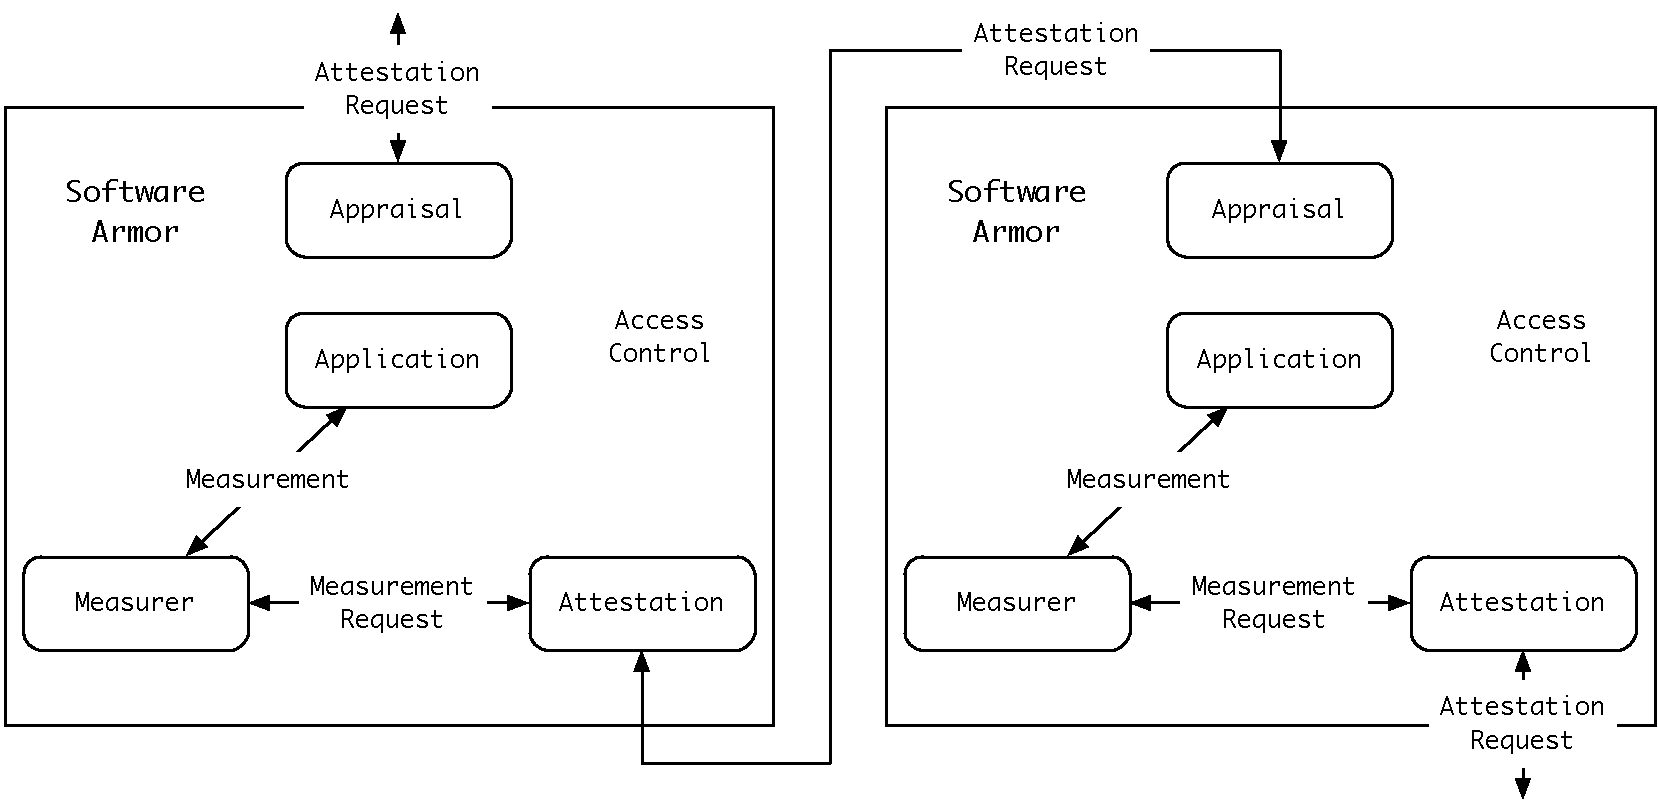
\includegraphics[width=0.85\textwidth]{figures/system.pdf}
  \caption{Typical interaction among armored components with an
    appraiser interacting with an attestation agent to gather
    information.}
  \label{fig:system}
\end{figure}

\bibliography{onePager}

\end{document}
